\documentclass[12pt,tikz]{standalone}

\ifstandalone%
    \usepackage{import}%
    \import{../configuration/}{comon_packages.tex}%
    \import{../configuration/}{variables.tex}%
    \import{../configuration/}{conftikz.tex}%
    \import{../configuration/}{custom_config.tex}%
\fi

\begin{document}
  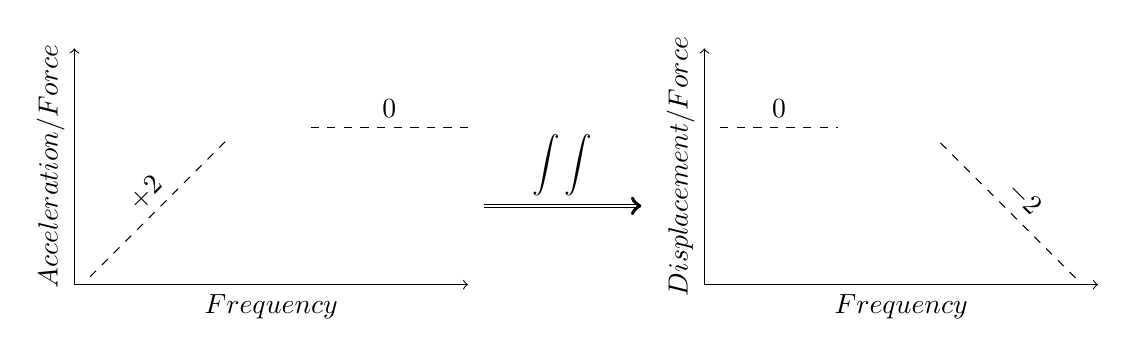
\begin{tikzpicture}
    \begin{scope}
      \draw[->] (0, 0) -- node[midway, below]{$Frequency$} (5, 0);
      \draw[->] (0, 0) -- node[midway, above, rotate=90]{$Acceleration/Force$} (0, 3);

      \draw[dashed] (0.2, 0.1) -- node[midway, above, rotate=45]{$+2$} ++(45:2.5);

      \draw[dashed] (3, 2) -- node[midway, above]{$0$} ++(0:2);
    \end{scope}

    \draw[->, double] (5.2, 1) -- node[midway, above]{$\displaystyle \int \int$} ++(2, 0);

    \begin{scope}[shift={(8, 0)}]
      \draw[->] (0, 0) -- node[midway, below]{$Frequency$} (5, 0);
      \draw[->] (0, 0) -- node[midway, above, rotate=90]{$Displacement/Force$} (0, 3);

      \draw[dashed] (0.2, 2) -- node[midway, above]{$0$} ++(0:1.5);

      \draw[dashed] (3, 1.8) -- node[midway, above, rotate=-45]{$-2$} ++(-45:2.5);
    \end{scope}
  \end{tikzpicture}
\end{document}
